
\setcounter{secnumdepth}{4}

\titleformat{\paragraph}
{\normalfont\normalsize\bfseries}{\theparagraph}{1em}{}
\titlespacing*{\paragraph}
{0pt}{3.25ex plus 1ex minus .2ex}{1.5ex plus .2ex}


\section{LPP for Optimization of Assets}

Linear Programming is the famous method used for the optimization of a given objective function and constraints. In this section we will use this method for the macro optimization of assets with respect to liabilities to ensure the liquidity risk. 

%\subsection{Prior Work}

\section{Algorithm}
The algorithm for the LPP optimization using simplex method is as follows:


\begin{algorithm}[H]

\caption{The Algorithm for LPP Optimization}

\begin{algorithmic}[1] 
						
\STATE Objective Function: \begin{equation}Maximize  Profit =  \Sigma_{j=1}^{m} Asset_{j} -  \Sigma_{i=1}^{n} Liability_{i}\end{equation}\\
		which can further be simplified as\\
		\begin{equation}Maximize  G_{b} =  \sum_{a=1}^{k-1} \sum_{c=1}^{m} \{ Y_{c}^{a,b} + Y_{c}^{a,b} * IA_{c}^{a,b} * TA_{c}^{a,b} \} -  \sum_{a=1}^{k-1} \sum_{d=1}^{n} \{ X_{d}^{a,b} + X_{d}^{a,b} * IL_{d}^{a,b} * TL_{d}^{a,b}\} \end{equation}

\STATE Assumption: \\a. No amount is expected to be paid or received from previous time buckets as there are no assets and liabilities in previous time bucket.\\
b. We have 5 assets and 5 liabilites.
	
\STATE Constraints : \\

For First Time Bucket: 
\begin{equation} X_{1}^{1,3} + X_{2}^{1,4} + X_{3}^{1,5} +X_{4}^{1,5} + X_{5}^{1,6} + X_{1}= Y_{1}^{1,2} + Y_{2}^{1,3} +Y_{3}^{1,5} + Y_{4}^{1,6}\end{equation}

For Second Time Bucket:
\begin{equation}
[Y_{1}^{1,2} + Y_{1}^{1,2}* IA_{1}^{1,2} * TA_{1}^{1,2}] +  X_{1}^{2,4} + X_{2}^{2,4} + X_{3}^{2,5} + X_{4}^{2,6} + X_{5}^{2,7} + G_{2} = Y_{1}^{2,3} + Y_{2}^{2,4} +  Y_{3}^{2,5} +  Y_{4}^{2,7} +  Y_{5}^{2,7} 
\end{equation}

and so on until we have time buckets left.

\STATE Convert constraint inequality to equality by adding slack variables to the constraints.

\STATE Use objective function and constraints of LPP to create initial Simplex table.

\STATE Find out initial solution by assigning 0 to decision variable

\STATE Optimality Test: \\ 
\tab a. Calculate	c$_{j}$ - z$_{j}$  \\ 
\tab b. If the calculated values are positive then optimal solution is the current basic solution. The greatest value column is the key column.\\ 
\tab c. If any one value is negative then choose the greatest value corresponding variable.

\STATE Feasibility Test: \\
\tab Computr the ratios by dividing the value under XB Column by corresponding valueo of key column.  The minimum value of ratio identifies the key row. 

\STATE Key Element:\\
\tab The intersection of key column and key roe gives the key element.

\STATE Updating the Table:
\tab a. For key row use formula \begin{equation}
New\_Value = \frac{Old\_Value}{Key\_Value}
\end{equation}
\tab b. For Other rows use formula:\\

New\_Value = Old\_Value - $\frac{Corresponding\_key\_column\_value *  corresponding \_key\_row\_value}{Key\_Value}$ \\

\STATE Repeat step 7 to 10 until all the values of c$_{j}$ - z$_{j}$ are 0 or negative.

\end{algorithmic}

\end{algorithm}


\section{Illustration}

				\begin{center}
				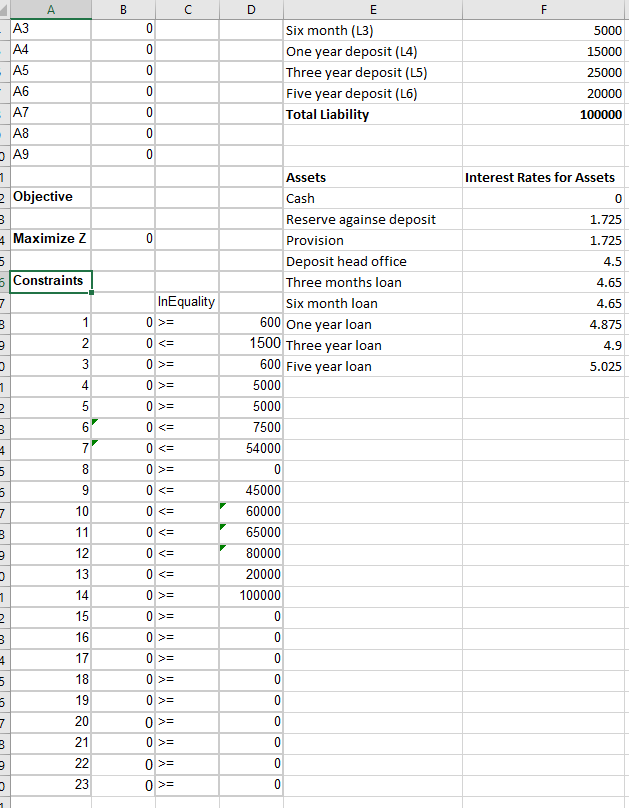
\includegraphics[width=\linewidth]{figures/LPP-Problem.jpg}	
				\captionof{figure}{LPP Problem Formulation in Excel}
				\label{fig: LPP Problem Formulation in Excel}
				\end{center}

				\begin{center}
				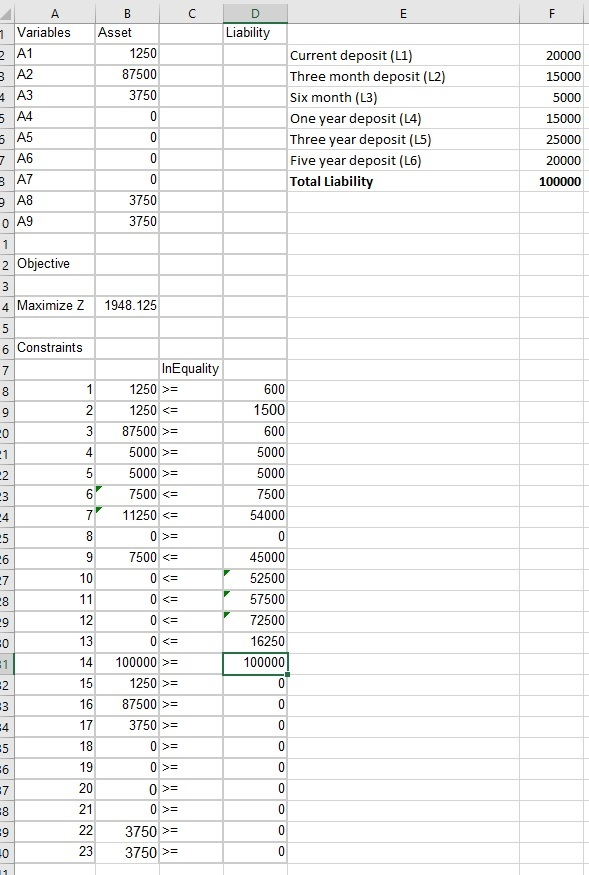
\includegraphics[width=\linewidth]{figures/LPP-Solution.jpg}	
				\captionof{figure}{LPP Problem Solution in Excel}
				\label{fig: LPP Problem Solution in Excel}
				\end{center}

\section{Computational Complexity}
The worst case complexity of Simplex Method is Exponential but in practice it's complexity is in polynomial time.

\section{Conclusion }
In this chapter we have addressed the problem of liquidity risk management using single objective optimization method.








